\documentclass[11pt]{article}

\usepackage[utf8]{inputenc}
\usepackage[T1]{fontenc}
\usepackage{lmodern}
\usepackage{ngerman}
\usepackage{graphicx}
\usepackage{textcomp}
\usepackage{units}
\usepackage{float}

\title{G"ansebl"umchen\\
	\begin{figure}[H]
	    \centering
        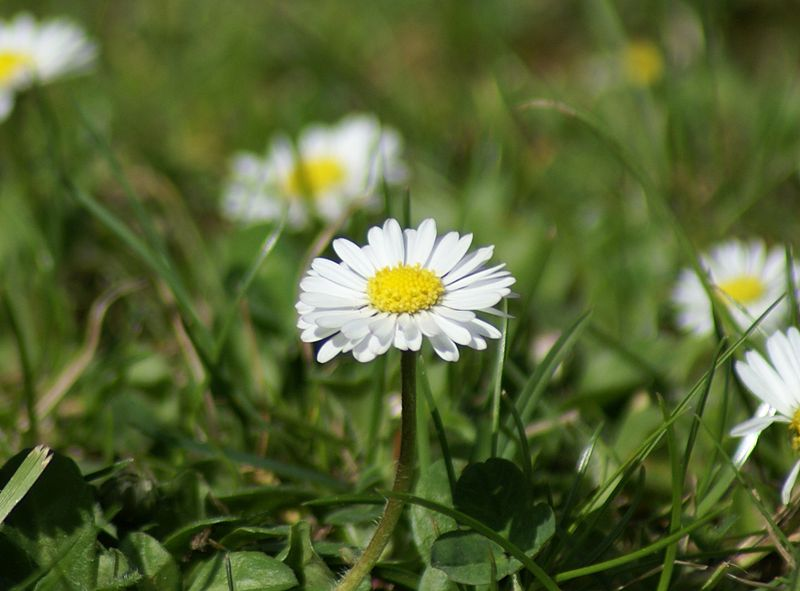
\includegraphics[width=0.66\textwidth]{1.jpg}
    	\caption{Gänseblümchen (Bellis perennis)}
	    \label{fig1}
    \end{figure}
    }  
\author{Evelyn Jochim und Jonjer Jennerjahn }          
\date{15. November bis 13. Dezember 2016}

\begin{document}
  
    \maketitle 
    \thispagestyle{empty}
    \newpage
	\tableofcontents
	\thispagestyle{empty}
	\newpage
	
	\section*{Vorwort}
	Dies geschieht im Rahmen der Veranstaltung: Werkzeuge für das wissenschaftliche Arbeiten
	
	\section{Abstract}
	Bellis perennis is a common European species of daisy, of the Asteraceae family, often considered the archetypal species of that name.
    Many related plants also share the name daisy , so to distinguish this species from other daisies it is sometimes qualified as common daisy, lawn daisy or English daisy. Historically, it has also been commonly known as bruisewort and occasionally woundwort (although the common name woundwort is now more closely associated with Stachys (woundworts)). Bellis perennis is native to western, central and northern Europe, but widely naturalised in most temperate regions including the Americas\cite{2}\cite{3} and Australasia.



	\section{Kurzfassung}
	Das Gänseblümchen (Bellis perennis), auch Ausdauerndes Gänseblümchen,\cite{1} Mehrjähriges Gänseblümchen, Maßliebchen, Tausendschön, Monatsröserl oder schweizerisch Margritli („Kleine Margerite“) genannt,\cite{2} ist eine Pflanzenart innerhalb der Familie der Korbblütler (Asteraceae). Da es auf fast jeder Wiesenfläche wächst, zählt es zu den bekanntesten Pflanzenarten Mitteleuropas.
	
	\begin{figure}[H]
	    \centering
        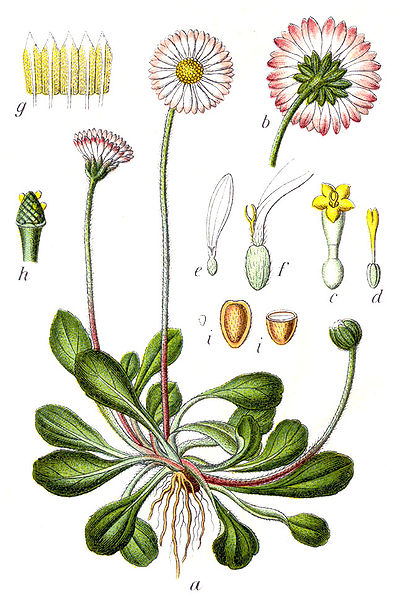
\includegraphics[width=0.66\textwidth, angle=30]{2.jpg}
    	\caption{Illustration von Johann Georg Sturm}
	    \label{fig2}
    \end{figure}
	
	\section{Einleitung}
	In dieser Bachelorarbeit beschäftigen wir uns mit Gänseblümchen.  
	    
	
	\section{Zusammenfassung}
	Dies war ein Bericht über Gänseblümchen. 
	
	\section{Beschreibung}
	\subsection{Erscheinungsbild und Blatt}
	Das Gänseblümchen ist eine ausdauernde, krautige Pflanze, die Wuchshöhen von meist 4 bis 15 (2 bis 20)\cite{2} Zentimetern erreicht. Am kurzen, aufrechten Rhizom befinden sich faserige Wurzeln.\cite{3}
    Die in einer dichten Blattrosette zusammen stehenden Laubblätter sind in Blattstiel und Blattspreite gegliedert. Der geflügelte Blattstiel ist mindestens so lang wie die Blattspreite.\cite{3} Die einfache Blattspreite besitzt nur einen Mittelnerv, ist spatelförmig bis verkehrt-eiförmig,\cite{2} 6 bis 40 Millimeter lang und 4 bis 20 Millimeter breit.\cite{3}

	\subsection{Blütenstand und Blüte}
	Jede Blattrosette bringt von März bis November ununterbrochen aufsteigende bis aufrechte, blattlose, meist 5 bis 15 (3 bis 20) Zentimeter\cite{3} lange Blütenstandsschäfte mit einzeln stehenden Blütenkörbchen hervor.\cite{2}
    Der körbchenförmige Blütenstand enthält Hüllblätter, die einen bewimperten Rand besitzen. Die mehr als hundert Blüten sind – wie für Korbblütler typisch – auf der verbreiterten Sprossachse, dem so genannten Blütenstandsboden angeordnet.\cite{3} Randständig sind die weißen, zygomorphen, weiblichen, 4 bis 8 (bis 11) mm\cite{3} langen Zungenblüten in zwei Reihen angeordnet. Im Zentrum des Blütenkörbchens stehen zwischen 75 und 125 gelbe, zwittrige und trichterförmige radiärsymmetrische, 1,5 mm lange\cite{3} Röhrenblüten. Zwei Fruchtblätter sind zu einem unterständigen, einfächrigen Fruchtknoten verwachsen.

	\subsection{Frucht}
	Die Früchte sind nicht wie jene vieler Arten der Korbblütengewächse mit einem Pappus ausgestattet. Bei den 1 bis 2 mm langen Achänen\cite{3} handelt es sich um gekrönte Schließfrüchte, bei der Frucht- und Samenschale miteinander verwachsen sind. Die Samen sind endospermlos.
	
	\subsection{Chromosomensatz}
	Die Chromosomenzahl beträgt 2n = 18.\cite{2}
	
	\section{Ökologie}
	Was für einen Laien wie eine einzige Blüte aussieht, ist tatsächlich eine Scheinblüte (Pseudanthium). Das Blütenkörbchen richtet sich aufgrund des Heliotropismus immer nach der Sonne und schließt sich abends sowie bei schlechtem Wetter. Die Blütenkörbchen von Bellis perennis, welche von Februar bis in den November hinein aufblühen, werden von Bienen, Hummeln, Schwebfliegen und vor allem Fliegen besucht. Zum Teil findet bei diesen Blütenbesuchen Fremdbestäubung statt. Auch verhilft dies zu einer Form der Selbstbestäubung, der sogenannten Geitonogamie, d. h. die einzelnen Blüten innerhalb eines Blütenköpfchens bestäuben sich gegenseitig. Die Selbstbestäubung innerhalb einer Einzelblüte (Autogamie) ist fraglich, jedoch nicht gänzlich ausgeschlossen. Die Blüten sind, wie für Korbblütler typisch, vormännlich, das heißt, die Staubblätter sondern reife Pollen ab, wenn die in der Blüte befindlichen Fruchtblätter noch nicht bereit für eine Bestäubung sind. Bei bestäubten Blüten entwickelt sich aus dem Fruchtknoten ein Nüsschen, die sogenannte Achäne. Das Gänseblümchen nutzt eine Reihe sehr unterschiedlicher Strategien zur Ausbreitung dieser Achänen.
    Typisch für Gänseblümchen ist die Verbreitung der Achänen durch den Regen. Dadurch werden die Achänen im Umkreis der Mutterpflanze von ihr weggeschleudert. Eine andere Ausbreitungsform findet durch den Wind statt (Anemochorie). Die elastischen und etwas verlängerten Stängel werden durch Windböen bewegt und die kleinen Achänen ausgestreut. Die Achänen werden aber auch durch Tiere verbreitet (Zoochorie), vor allem durch Regenwürmer, Schafe und Rinder. Schließlich hilft sogar der Mensch bei der Ausbreitung (Anthropochorie). Das Gänseblümchen vermehrt sich generativ durch Samen (Achänen) und vegetativ.
    
    \section{Vorkommen}
    \dots 
    
    \section{Taxonomie}
    \dots
    
    \section{Gänseblümchen und Mensch}
    \subsection{Trivialnamen}
    Diese weit verbreitete Pflanzenart trägt eine Reihe von volkstümlichen Namen, die regional sehr unterschiedlich sein können. Typisch sind Angerbleamerl, Augenblümchen, Himmelsblume, Maiblume, Marienblümchen, Maßliebchen, Mondscheinblume, Morgenblume, Osterblume, Regenblume, Sommerröschen,\cite{6} Sonnenblümchen und Tausendschön. In der Schweiz auch: Gisegeisseli, Geissemeieli, Geisseblüemli,\cite{7} \dots
    
    \subsection{Verwendung als Nahrungspflanze}
	\dots 
	
	\subsection{Pharmazie- und Botanikgeschichte}
	\dots 
	In einem Elsässer Manuskript aus dem 1. Viertel des 15. Jh. wurde das Gänseblümchen „Citelosen“ genannt: „Citelosen wasser von dem krute gebrant getruncken ist den wunden luten gut vnd heilet dz verserte gederme vnd machet weich in dem libe.“\cite{13}
	\dots 
	
	
\bibliographystyle{plain}
\bibliography{gaense}
\end{document}